%\documentclass{article}
%\usepackage{graphicx,subfigure}
%\begin{document}

\begin{figure}[h]
  \centering
   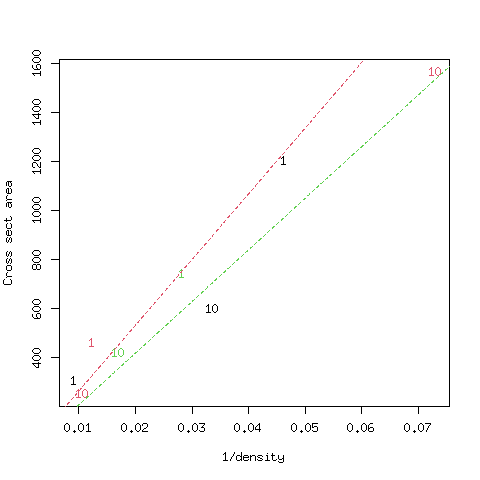
\includegraphics[width=0.9\textwidth]{DC1955/expt3reg.png}
  \caption{Plot of breed means for reciprocal of follicle density and fibre cross sectional area from Daly and Carter(1956)~\cite{daly:56} experiment 3.  The red lines are linear regressions  with zero intercept fitted to breed means for period 1 (lowest liveweight). The green lines are linear regressions with zero intercept fitted to breed means for period 10 (higher liveweight and older).}
  \label{fig:dcexpt3reg}
\end{figure}

%\end{document}

